% !TeX root = ../main.tex

\section{Hilbert Space}

\begin{problem}[Function space]
  A square-integrable function, or $L^2$ function, is a real- or complex-valued
  function for which the integral of the square of the absolute value is finite.
  Let us consider the set of complex-valued, continuous $L^2$ functions on the real line $\mathbb R$ (or on a subset $A \subset \mathbb R$).
  The set $L^2(A) = \{\psi: A \to \mathbb C | \int_A |\psi(x)|^2 \d x < \infty\}$
  is naturally a complex vector space, called \emph{function space}.
  \begin{enumext}
    \item Show that the integral $\int_A \varphi(x)^* \psi(x) \d x$
    with $\varphi$, $\psi \in L^2(A)$ defines an \emph{inner product}
    $\braket<\varphi|\psi>$.
    \item $L^2(A)$ is a Hilbert space with the above definition of inner product.
    Find at least two different orthonormal bases (excluding $\delta$-functions)
    for each of the three cases
    \begin{enumext}[columns = 3]
      \item $A = (-\infty, +\infty)$;
      \item $A = [-1, 1]$;
      \item $A = (0, +\infty)$.
    \end{enumext}
    Demonstrate the orthonormality and the completeness explicitly.
    (Hint: One choice can be our familiar Fourier basis
    and the other from a polynomial expansion by virtue of
    \emph{Weierstrass's theorem}). Also see Problem 1.2.
  \end{enumext}
\end{problem}
\begin{solution}\leavevmode
  \begin{enumext}
    \item \begin{proof}
    To show that the integral defines an inner product, we check the axioms of an inner product on a complex vector space.
    \begin{enumext}
      \item Conjugate symmetry: $\braket<\varphi|\psi> = \int_A \varphi^*\psi
      = \overline{\int_A \psi^*\varphi} = \overline{\braket<\psi|\varphi>}$.
      \item Linearity: For $\alpha$, $\beta \in \mathbb C$,
      in the second argument,
      \[
        \braket<\varphi|(\alpha\psi_1 + \beta\psi_2)>
      = \int_A \varphi^*(\alpha\psi_1 + \beta\psi_2)
      = \alpha\braket<\varphi|\psi_1> + \beta\braket<\varphi|\psi_2>.
      \]
      Conjugate-linearity in the first argument follows similarly.
      \item Positive-definiteness: $\braket<\psi|\psi> = \int_A |\psi(x)|^2 \d x\geq 0$, also for $\varphi$.
    \end{enumext}
    Hence, $\braket<\varphi|\psi>$ is an inner product on $L^2(A)$.
    \end{proof}
    \item \begin{enumext}
      \item $A = (-\infty, +\infty)$
      \begin{enumext}[wrap-label = \underline{Case #1}, label = \arabic*,
                      list-indent = 0pt]
        \item Hermite functions
        \[
          \psi_n(x) = \frac1{\sqrt{\sqrt\pi2^nn!}} H_n(x) \upe^{-x^2/2}, \quad
          n = 0,1,2,\ldots,
        \]
        where $H_n$ is the $n-$th Hermite polynomial, belong to $L^2(\mathbb R)$.
        Using the orthonormality of the Hermite polynomial,
        we get the orthonormality of the function
        \[
          \int_A \psi_m(x) \psi_n(x) \d x = \delta_{mn}.
        \]
        From Sturm-Liouville theory,
        $\{\psi_n\}_{n\geq0}$ form a basis for $L^2(\mathbb R)$.
        So it is complete.
        \item Haar basis
        \[
          \psi_{n,k}(x) = 2^{n/2} \psi_{0,0}(2^nx - k), \quad x \in \mathbb R,
        \]
        $\psi$ is a compactly supported mother wavelet chosen so that the  family is orthonormal in $L^2(\mathbb R)$
        \[
          \int_A \psi_{n,k}(x) \psi_{n',k'}(x) \d x = \delta_{nn'}\delta{jj'}.
        \]
        The Haar system on the real line is an orthonormal basis in $L^2(\mathbb R)$, so it is complete.
      \end{enumext}
      \item $A = [-1, 1]$
      \begin{enumext}[wrap-label = \underline{Case #1}, label = \arabic*,
                    list-indent = 0pt]
        \item Fourier basis
        \[
          \psi_n(x) = \frac1{\sqrt2} \upe^{\iu n\pi x}, \quad n \in \mathbb Z,
        \]
        its orthonormality
        \[
          \int_{-1}^1 \psi_m(x) \psi_n(x) \d x
        = \frac12 \int_{-1}^1 \upe^{\iu(m-n)\pi x} \d x = \delta_{mn},
        \]
        It is standard Fourier series theory, which satisfies completeness.
        \item Legendre polynomials
        \[
          \psi_n(x) = \sqrt{n + \frac12} P_n(x), \quad n = 0, 1, 2, \ldots,
        \]
        its orthonormality
        \[
          \int_{-1}^1 \psi_m(x) \psi_n(x) \d x
        = \frac{2n + 1}{2} \int_{-1}^1 P_m(x) P_n(x) \d x = \delta_{mn}.
        \]
        Due to Weierstrass' theorem, polynomials are dense in $A$ in the sup norm, hence complete in $L^2$.
      \end{enumext}
      \item $A = (0, +\infty)$
      \begin{enumext}[wrap-label = \underline{Case #1}, label = \arabic*,
                      list-indent = 0pt]
        \item Laguerre functions
        \[
          \psi_n(x) = \upe^{-x/2} L_n(x), \qq{where}
          L_n(x) = \upe^x \odv*[n]{(x^n \upe^{-x})}x,
        \]
        its orthonormality
        \[
          \int_A \psi_m(x) \psi_n(x) \d x = \int_A \upe^{-x} L_m(x) \d x
        = \delta_{mn}.
        \]
        The Laguerre polynomials (with the $\upe^{x/2}$ factor) are eigenfunctions of a self-adjoint Sturm-Liouville operator on
        $(0, \infty)$ and form a complete orthonormal set in $L^2(0, \infty)$.
        \item Consider the mapping
        $\varphi: A \to (0,1)$, $t \mapsto \frac2\pi\arctan(t)$.
        Then use the sine functions in $x$-space
        \[
          \psi(x) = \sqrt2\sin(n\pi t(x)),
        \]
        it is trivial that sine functions are orthonormal and complete.
      \end{enumext}
    \end{enumext}
  \end{enumext}
\end{solution}

\newpage

\begin{problem}[Sturm-Liouville theory]
  Many physics problems involve second-order, linear differential equations
  of the general form: $\alpha(x) y'' + \beta(x) y' + \gamma(x) y = \lambda y$,
  where $\alpha$, $\beta$, and $\gamma$ are real functions, and $\lambda$ is a constant.
  Such an ODE can be rewritten in a \emph{Sturm-Liouville} form $\mathcal Ly = \lambda y$
  with a proper choice (cf. (a)) of the \emph{weight function} $\omega(x)$ in the linear second-order differential operator
  \[
    \mathcal L = \omega^{-1} \odv*{\ab(\omega \alpha \odv*{}x)}x + \gamma.
  \]
  This, combined with suitable boundary conditions (cf. (b)), renders $\mathcal L$
  a self-adjoint operator if the inner product is defined to be
  \[
    \braket<u|v> = \int_{x_1}^{x_2} u^*(x) v(x) \omega(x) \d x.
  \]
  Hence, the Sturm-Liouville problem becomes an eigenvalue problem with the solutions being the eigenvalues and the corresponding $\lambda$'s being the eigenvalues.
  The Sturm-Liouville theory provides a connection between a second-order, linear differential equation and Hilbert space $\mathcal L^2 ([x_1, x_2])$
  by establishing the normalized eigenvectors of the former (in its Sturm-Liouville form) as a complete orthonormal basis of the latter.
  \begin{enumext}
    \item Find the general expression of $\omega(x)$ that permits the rewriting of the original ODE in its Sturm-Liouville form.
    Compute $\omega(x)$ for the following ODEs
    \begin{alignat*}{4}
      & \qq{(i)}   && -y'' + 2xy' = \lambda y         && \qq{(Hermite)}\\
      & \qq{(ii)}  && -(1 - x^2)y''+ 2xy' = \lambda y && \qq{(Legendre)}\\
      & \qq{(iii)} && -xy'' - (1 - x)y' = \lambda y   && \qq{(Laguerre)}
    \end{alignat*}
    \item Find the general boundary condition $\mathcal L$
    to be self-adjoint in $[x_1, x_2]$ with respect to the above-defined inner product,
    namely, $\braket<u|\mathcal Lv> = \braket<\mathcal Lu|v>$.
    Note that $u$ and $v$ can, in general, be complex functions.
    Check that the boundary condition is satisfied when
    \begin{enumext}
      \item $x_1 = -\infty$, $x_2 = +\infty$ for Hermite equation.
      \item $x_1 = -1$, $x_2 = 1$ for Legendre equation.
      \item $x_1 = 0$, $x_2 = +\infty$ for Laguerre equation.
    \end{enumext}
    \item With $\mathcal L$ being self-adjoint in $[x_1, x_2]$, show that if
    $\mathcal Lv_i = \lambda_i v_i$ ($i = 1$, $2$) and $\lambda_1 \neq \lambda_2$,
    then $\braket<v_1|v_2> = 0$.
  \end{enumext}
\end{problem}
\begin{solution}\leavevmode
  \begin{enumext}
    \item Apply $\mathcal L$ to a test function $y$, we have
    \[
      \mathcal Ly = \frac1\omega[(\omega\alpha)'y' + \omega\alpha y''] + \gamma y
    = \alpha y'' + \frac{(\omega\alpha)'}{\omega}y' + \gamma y,
    \]
    Comparing with the original $\alpha y'' + \beta y' + \gamma y$, we require
    \[
      \beta(x) = \frac{(\omega\alpha)'}{\omega} = \alpha'(x) + \alpha(x) \frac{\omega'(x)}{\omega(x)}.
    \]
    Then, we can solve $\omega'/\omega$
    \[
      \frac{\omega'}{\omega} = \frac{\beta(x) - \alpha'(x)}{\alpha(x)},
      \quad
      \omega(x) = C \exp\ab(\int_A \frac{\beta(x') - \alpha'(x')}{\alpha(x')} \d x'),
    \]
    where $C$ is an arbitrary positive constant,
    and $A$ is the integral range for the following different types.
    \begin{enumext}[wrap-label* = \underline{\emph{#1}}, list-indent = 0pt]
      \item [Hermite: $-y'' + 2xy' = \lambda y$]\leavevmode\\
      To compare with, we have $\alpha = -1$, $\beta = 2x$, $\alpha' = 0$. Then
      \[
        \omega'/\omega = (2x - 0)/(-1) = -2x, \quad
        \omega(x) = C \upe^{-x^2}.
      \]
      \item [Legendre: $-(1 - x^2)y'' + 2xy' = \lambda y$]\leavevmode\\
      To compare with, we have $\alpha = -(1 - x^2)$, $\beta = 2x$, $\alpha' = 2x$.
      Then
      \[
        \omega'/\omega = (2x - 2x)/(-1), \quad \omega(x) = C.
      \]
      \item [Laguerre: $-xy'' - (1 - x)y' = \lambda y$]\leavevmode\\
      To compare with, we have
      $\alpha = -x$, $\beta = -(1 - x) = x - 1$, $\alpha' = -1$. Then
      \[
        \omega'/\omega
      = [(x - 1) - (-1)]/(-x) = -1, \quad \omega(x) = C \upe^{-x}.
      \]
    \end{enumext}
    \item Using the inner product
    \[
      \braket<u|v> = \int_{x_1}^{x_2} u^*(x) v(x) \omega(x) \d x.
    \]
    to compute the difference $\braket<u|\mathcal Lv> - \braket<\mathcal Lu|v>$.
    We have
    \begin{align*}
      \braket<u|\mathcal Lv> & = \int_{x_1}^{x_2}
      u^* \ab[\omega^{-1} (\omega \alpha v')' + \gamma v] \omega \d x
    = \int_{x_1}^{x_2} u^* (\omega \alpha v')' \d x
    + \int_{x_1}^{x_2} u^* v \gamma \omega \d x,\\
      \braket<\mathcal Lu|v> & = \int_{x_1}^{x_2}
      \ab[\omega^{-1} (\omega \alpha (u^*)' )' + \gamma u^*] v \omega \d x
    = \int_{x_1}^{x_2} (\omega \alpha (u^*)')' v \d x
    + \int_{x_1}^{x_2} \gamma u^* v \omega \d x.
    \end{align*}
    Then the difference can be expressed as
    \[
      \braket<u|\mathcal Lv> - \braket<\mathcal Lu|v>
    = \ab[\omega(x) \alpha(x) (u^*(x) v'(x) - u'^*(x) v(x))]_{x_1}^{x_2}.
    \]
    If it is zero, then $\mathcal L$ is adjoint under the corresponding interval.
    Now, substitute the three boundary conditions into the difference.
    \begin{enumext}
      \item Hermite: $x \in (-\infty, +\infty)$, $\omega = e^{-x^2}$, $\alpha = -1$.
      Boundary term: $[-e^{-x^2} (u^* v' - u'^* v)]_{-\infty}^{+\infty} = 0$.
      \item Legendre: $x \in [-1, 1]$, $\omega = 1$, $\alpha = -(1 - x^2)$.
      Boundary term $\ab[-(1 - x^2) (u^* v' - u'^* v)]_{-1}^1 = 0$.
      \item Laguerre: $x \in [0, \infty)$, $\omega = e^{-x}$, $\alpha = -x$.
      Boundary term $\ab[-x e^{-x} (u^* v' - u'^* v)]_0^{\infty} = 0$.
    \end{enumext}
    So, $\mathcal L$ is self-adjoint in the three domain.
    \item \begin{proof}
    Using self-adjointness for $i = 1$ and $i = 2$
    \[
      \lambda_2 \braket<v_1|v_2> = \braket<v_1|\mathcal L v_2>
    = \braket<\mathcal L v_1|v_2> = \lambda_1 \braket<v_1|v_2>.
    \]
    Rearranging, we can obtain
    \[
      (\lambda_2 - \lambda_1) \braket<v_1 | v_2> = 0.
    \]
    Since $\lambda_1 \neq \lambda_2$, then $\braket<v_1|v_2> = 0$.
    \end{proof}
  \end{enumext}
\end{solution}

\newpage

\begin{problem}[Linear map]
  Let $V$ and $W$ be vector spaces over the same field $\mathbb K$.
  A map $f: V \to W$ is called a \emph{linear map} if $f(au + bv) = af(u) + bf(v)$
  for all $a$, $b \in \mathbb K$ and $u$, $v \in V$.
  \begin{enumext*}[label = (\alph*)]
    \item Show that the set $L(V,W)$ of linear maps from $V$ to $W$ itself forms a vector space over $\mathbb K$.
    \item Consider finite dimensional vector spaces $V$ and $W$.
    Let $\{v_1, v_2, \ldots, v_n\}$ be a basis of $V$, and
    $\{w_1, w_2, \ldots, w_n\}$ be a basis of $W$.
    Does the set of equations $f(v_i) = \sum_{j=1}^m \omega_j F_{ji}$
    with $i = 1, 2, \ldots, n$ and $F_{ij} \in \mathbb K$ uniquely determine
    the $m \times n$ matrix $F$? Why? Conversely, does any $m \times n$ matrix $F$
    over $\mathbb K$ uniquely determine a linear map $f$ by the same set of equations? Why?
    \item Following (a) and (b), find a basis of $L(V, W)$.
    \item* (optional) Define the \emph{kernel} of $f$ to be
    $\ker(f) = \{v \in V | f(v) = 0\}$ and the \emph{image} of $f$ to be
    $\im(f) = \{\omega \in W | \omega = f(v), v \in V\}$.
    Both the kernel and the image of $f$ are vector spaces with their dimensions
    called $\text{\emph{nullity}} = \dim(\ker(f))$ and $\rank = \dim(\im(f))$, respectively.
    Prove that
    \[
      \dim(\ker(f)) + \dim(\im(f)) = \dim(V).
    \]
  \end{enumext*}
\end{problem}
\begin{solution}\leavevmode
  \begin{enumext}
    \item \begin{proof}
    Define addition and scalar multiplication on $L(V,W)$ by
    \[
      (f + g)(v) = f(v) + g(v), \quad (\alpha f)(v) = \alpha (f(v)),
    \]
    for all $f,g \in L(V,W)$, $\alpha \in \mathbb{K}$, $v \in V$.
    \paragraph{Closure and linearity}
    If $f, g$ are linear, then for all $a,b \in \mathbb{K}$ and $u,v \in V$,
      \[
      (f+g)(a u + b v) = f(a u + b v) + g(a u + b v)
    = a (f + g)(u) + b (f + g)(v),
      \]
      so $f + g$ is linear. Similarly,
      \[
        (\alpha f)(a u + b v) = \alpha (f(a u + b v)) = \alpha (a f(u) + b f(v))
      = a (\alpha f)(u) + b (\alpha f)(v),
      \]
      so $\alpha f$ is linear.
    \paragraph{Vector space axioms}
    Associativity, commutativity of addition, existence of the zero map $0: V \to W$ with $0(v) = 0_W$, additive inverses $(-f)(v) = -f(v)$, and scalar multiplication axioms all follow from the corresponding properties in $W$.
    Thus $L(V, W)$ is a vector space over $\mathbb{K}$.
    \end{proof}
    \item Let $\dim V = n$ with basis $\{v_1, \dots, v_n\}$, and $\dim W = m$ with basis $\{w_1, \dots, w_m\}$, then
    \[
    f(v_i) = \sum_{j=1}^m F_{ji}  w_j, \quad i = 1, \dots, n.,
    \]
    which defines an $m \times n$ matrix $F = (F_{ji})$.
    \begin{enumext}
      \item For fixed $i$, the coefficients $F_{1i}, \dots, F_{mi}$ are the unique coordinates of $f(v_i)$ in the basis $\{w_j\}$. So $f(v_i) = \sum_j F_{ji} w_j$ uniquely determine $F$.
      \item Define $f$ on basis vectors by $f(v_i) = \sum_{j=1}^m F_{ji} w_j$, and extend linearly: for $v = \sum_{i=1}^n a_i v_i$, define
      \[
      f(v) = \sum_{i=1}^n a_i f(v_i) = \sum_{i=1}^n \sum_{j=1}^m a_i F_{ji} w_j.
      \]
      This is well-defined and linear, and uniquely determined by $F$.
      So, any $m \times n$ matrix $F$ uniquely determine a linear map $f$,
      and there is a bijection between $L(V,W)$ and $m \times n$ matrices over $\mathbb{K}$ once bases are fixed.
    \end{enumext}
    \item Under the identification $L(V,W) \cong \mathbb{K}^{m \times n}$, define for each $1 \le p \le m$, $1 \le q \le n$ the linear map $E^{(p,q)} : V \to W$ by
    \[
      E^{(p,q)}(v_q) = w_p, \quad E^{(p,q)}(v_k) = 0 \qq{for} k \ne q,
    \]
    extended linearly.
    The matrix of $E^{(p,q)}$ has a 1 in the $(p,q)$ entry and 0 elsewhere.  
    These $mn$ maps are linearly independent and span $L(V, W)$, hence form a basis.  
    Thus
    \[
      \dim L(V,W) = m n = \dim V \cdot \dim W.
    \]
    \item \begin{proof}
    Let $f : V \to W$ be linear, $\dim V = n$; and
    let $\dim(\ker f) = k$, and choose a basis $\{u_1, \dots, u_k\}$ of $\ker f$.  
    Extend to a basis $\{u_1, \dots, u_k, u_{k+1}, \dots, u_n\}$ of $V$.
    Let $S = \{f(u_{k+1}), \dots, f(u_n)\} \subset \im f$.
    \paragraph{Span}
    For any $v \in V$, write $v = \sum_{i=1}^n a_i u_i$. Then
    \[
      f(v) = \sum_{i=1}^n a_i f(u_i) = \sum_{i=k+1}^n a_i f(u_i),
    \]
    since $f(u_1) = \dots = f(u_k) = 0$. So $\im f \subseteq \operatorname{span}(S)$.
    \paragraph{Linear independence}
    Suppose $\sum_{i=k+1}^n b_i f(u_i) = 0$. Then
    \[
      f\ab(\sum_{i=k+1}^n b_i u_i) = 0,
    \]
    so $\sum_{i=k+1}^n b_i u_i \in \ker f$.  
    Since $\{u_1, \dots, u_k\}$ is a basis of $\ker f$
    \[
      \sum_{i=k+1}^n b_i u_i = \sum_{i=1}^k c_i u_i,
    \]
    for some $c_i$. By linear independence of the full basis, all $b_i = 0$.  
    So $S$ is linearly independent.
    Thus $S$ is a basis of $\im f$, and $|S| = n - k$.  
    Hence
    \[
      \dim(\ker f) + \dim(\im f) = k + (n - k) = n = \dim V.
    \]
    which is the rank-nullity theorem.
    \end{proof}
  \end{enumext}
\end{solution}

\newpage

\begin{problem}[Coherent states]
  A coherent state $\ket|\alpha>$ is defined as an eigenstate of the annihilation
  operator $\hat a$ with a complex eigenvalue $\alpha$:
  \[
    \hat a \ket|\alpha> = \alpha \ket|\alpha>.
  \]
  \begin{enumext}
    \item Show that $\ket|\alpha> = \mathcal N\upe^{\alpha \hat a^\dagger} \ket|0>$,
    where $\mathcal N$ is a normalization constant and $\ket|0>$ is the ground state such that $\hat a\ket|0> = 0$ (review the solution of a quantum harmonic oscillator if needed).
    Compute $\mathcal N$ and $\braket<\alpha|\hat a^\dagger \hat a|\alpha>$.
    Further show that $\ket|\alpha> = \upe^{\alpha\hat a^\dagger-\alpha^*\hat a} \ket|0>$
    up to a phase factor.
    $D(\alpha) \equiv \upe^{\alpha\hat a^\dagger-\alpha^*\hat a}$
    is a unitary operator called the displacement operator because it displaces the ground state $\ket|0>$ to $\ket|\alpha>$ (note that $\ket|0>$ is a special coherent state with $\alpha = 0$).
    \item Show that the set $\{\ket|\alpha> | \alpha \in \mathbb C\}$
    form an overcomplete basis of the Hilbert space by computing
    $\braket<\alpha|\beta>$ for generic $\alpha$ and $\beta$, and proving
    \[
      \int \frac{\d^2\alpha}{\pi} \ketbra|\alpha><\alpha| = \mathbbm 1,
    \]
    where $\d^2\alpha = \d \Re\alpha \d\Im\alpha = r_\alpha \d r_\alpha\d \varphi_\alpha$ ($\alpha = \Re\alpha + \iu\Im\alpha = r_\alpha\upe^{\iu\varphi_\alpha}$).
    (Hint: Consider the matrix elements of the above operator in the orthonormal basis $\{\ket|n>\}$.)
    \item In the context of a quantum harmonic oscillator,
    $\hat a = (l^{-1}_0 \hat x + \iu l_0\hat k)/\sqrt2$,
    where $l_0 \equiv \sqrt{\hbar/m\omega}$.
    Find the wavefunction (in real space) of a coherent state $\braket<x|\alpha>$,
    and compare this wavefunction with the Gaussian wave packet we have learned in our class.
    (Hint: Consider the real-space representation of the defining equation $\hat a\ket|\alpha> = \alpha\ket|\alpha>$.)
    \item Compute $\hat U^{-1}(t,0) \hat a \hat U(t,0)$ with
    $\hat U(t,0) = \exp[-\iu(\hat a^\dagger\hat a + 1/2)\omega t]$,
    and use the result to derive $\hat U(t,0) \ket|\alpha>$.
    Interpret the result in the context of a quantum harmonic oscillator.
    (Hint: What is the physical meaning of $\Re\alpha$ and $\Im\alpha$?)
  \end{enumext}
\end{problem}
\begin{solution}\leavevmode
  \begin{enumext}
    \item \begin{proof}
    Expand the coherent state $\ket|\alpha>$ in terms of number state $\ket|n>$
    \[
      \ket|\alpha> = \sum_{n=0}^\infty c_n \ket|n>.
    \]
    Here, we merge the normalization factor into $c_n$ to simplify, and it will be released at the end. Act $\hat a$ on the expand expression of $\ket|\alpha>$, due to the property of annihilation operator
    \[
      \hat a \ket|\alpha> = \sum_{n=0}^\infty c_n \hat a \ket|n>
    = \sum_{n=1}^\infty c_n \sqrt n \ket|n - 1>
    = \alpha \sum_{n=0}^\infty c_n \ket|n>,
    \]
    the third term summing from $n = 1$ is due to $\hat a\ket|0> = 0$,
    which $n = 0$ make no sence. To uniform the lower limit of $n$,
    shift the summation index
    \[
      \hat a \ket|\alpha>
    = \sum_{n=0}^\infty c_{n+1} \sqrt{n + 1} \ket|n>
    = \alpha \sum_{n=0}^\infty c_n \ket|n>,
    \]
    then we obtain the expression of the expansion coefficient
    \[
      c_{n+1} \sqrt{n + 1} = \alpha c_n, \qq{or}
      c_n = \frac\alpha{\sqrt n} c_{n-1}
    = \frac\alpha{\sqrt n} \frac\alpha{\sqrt{n - 1}} c_{n-2} = \cdots
    = \frac{\alpha^n}{\sqrt{n!}} c_0,
    \]
    thus
    \[
      \ket|\alpha> = c_0 \sum_{n=0}^\infty \frac{\alpha^n}{\sqrt{n!}} \ket|n>
    = c_0 \sum_{n=0}^\infty \frac{(\alpha \hat a^\dagger)^n}{n!} \ket|0>
    = c_0 \upe^{\alpha \hat a^\dagger} \ket|0>,
    \]
    where $\ket|n> = \frac{(\hat a^\dagger)^n}{\sqrt{n!}}\ket|0>$.
    To get the expression of $c_0$, normalize it
    \[
      1 = \braket<\alpha|\alpha> = |c_0|^2
      \braket<0|\upe^{\alpha^*\hat a} \upe^{\alpha\hat a^\dagger}|0>
    = |c_0|^2 \sum_{n=0}^\infty \frac{|\alpha|^{2n}}{n!} \braket<n|n>
    = |c_0|^2 \upe^{|\alpha|^2}.
    \]
    Hence, we prove that
    \[
      \ket|\alpha> = \upe^{-|\alpha|^2/2} \upe^{\alpha \hat a^\dagger} \ket|0>
    = \mathcal N \upe^{\alpha \hat a^\dagger} \ket|0>,
    \]
    where $\mathcal N = c_0 = \upe^{-|\alpha|^2/2}$.
    And the ``exception value'' of $\hat a^\dagger \hat a$ under the coherent state
    \[
      \braket<\alpha|\hat a^\dagger \hat a|\alpha>
    = \alpha^*\alpha\braket<\alpha|\alpha> = |\alpha|^2,
    \]
    where $\bra<\alpha|\hat a^\dagger = \alpha^* \bra<\alpha|$.
    The displacement operator can be written as
    \[
      D(\alpha) = \upe^{\alpha \hat a^\dagger - \alpha^*\hat a}
    \xlongequal[{[\alpha\hat a^\dagger, -\alpha^*\hat a] = |\alpha|^2}]{\text{BCH identity}}
      \upe^{-|\alpha|^2/2} \upe^{\alpha \hat a^\dagger} \upe^{-\alpha^* \hat a},
    \]
    when it acts on the vacuum $\ket|0>$, to calculate it, we need to expand
    the last term $\upe^{-\alpha^* \hat a}$
    \[
      \upe^{-\alpha^* \hat a} \ket|0> = \sum_{k=0}^\infty \frac{(-\alpha^*)^k}{k!} \hat a^k \ket|0> = \ket|0>.
    \]
    Due to every $\hat a$ annihilates $\ket|0>$, so only the $k = 0$ term survives. So the result of the displacement operator acting on the vacuum is
    \[
      D(\alpha) \ket|0> = \upe^{-|\alpha|^2/2} \upe^{\alpha \hat a^\dagger} \ket|0> \equiv \ket|\alpha>.
    \]
    i.e., the overall phase convention.
    \end{proof}
    \item \begin{proof}
    Firstly, we need to calculate some identities for preparation.
    \begin{itemize}
      \item Verify $D(\alpha)$ is a unitary operator.
      \begin{equation}
        D^\dagger(\alpha) = \upe^{\alpha \hat a - \alpha^*\hat a^\dagger}
      = D(-\alpha) = D^{-1}(\alpha).\tag{A}
      \label{problem:2.4:A}
      \end{equation}
      \item Calculate $\braket<0|\upe^{\gamma \hat a^\dagger}|0>$
      \begin{equation}
        \braket<0|\upe^{\gamma \hat a^\dagger}|0>
      = \sum_{k=0}^\infty \frac{\gamma^k}{k!}\braket<0|(\hat a^\dagger)^k|0>
      = \frac{\gamma^0}{0!}\braket<0|0>
      + \sum_{k=1}^\infty \frac{\gamma^k}{k!} \sqrt{k} \braket<0|k> + \cdots
      = 1.\tag{B}
        \label{problem:2.4:B}
      \end{equation}
      Since $\braket<m|n> = \delta_{m,n}$, only $k = 0$ term survives.
      \item Calculate $\braket<m|\alpha>$ and $\braket<\alpha|n>$.
      Expand $\ket|\alpha>$ in terms of number basis
      \[
        \ket|\alpha> = \upe^{-|\alpha|^2/2} \upe^{\alpha \hat a^\dagger} \ket|0>
      = \upe^{-|\alpha|^2/2} \sum_{n=0}^\infty
        \frac{a^n}{n!} (\hat a^\dagger)^n \ket|0>
      \xlongequal[\text{Property of creation O.P.}]{(\hat a^\dagger)^n = \sqrt{n!}\ket|n>}
        \upe^{-|\alpha|^2/2} \sum_{n=0}^\infty
        \frac{a^n}{\sqrt{n!}} \ket|n>. 
      \]
      Now we obtain the inner product
      \begin{equation}
        \braket<m|\alpha> = \upe^{-|\alpha|^2/2} \sum_{n=0}^\infty
        \frac{a^n}{\sqrt{n!}} \delta_{mn}
      = \upe^{-|\alpha|^2/2} \frac{a^m}{\sqrt{m!}}, \qq{similarly}
      \braket<\alpha|n> = \upe^{-|\alpha|^2/2} \frac{(a^*)^n}{\sqrt{n!}}\tag{C}.
        \label{problem:2.4:C}
      \end{equation}
    \end{itemize}
    Now, calculate $\braket<\alpha|\beta>$. Write them in terms of the displacement operator
    \[
      \braket<\alpha|\beta> = \braket<0|D^\dagger(\alpha) D(\beta)|0>
    = \braket<0|D(-\alpha) D(\beta)|0>
    \xlongequal{\text{BCH identity}}
    \upe^{\frac12(\alpha^(\beta-\alpha\beta^*))} \braket<0|D(\beta - \alpha)|0>,
    \]
    where we used Eq. \eqref{problem:2.4:A}.
    Denote $\gamma = \beta - \alpha$ for simplification,
    using Eq. \eqref{problem:2.4:B}
    \[
      \braket<0|D(\beta - \alpha)|0> = \braket<0|D(\gamma)|0>
    \xlongequal{\text{BCH identity}} \upe^{-|\gamma|^2/2} \braket<0|\upe^{\gamma \hat a^\dagger}|0> = \upe^{-|\gamma|^2/2}.
    \]
    Substitute this equation to $\braket<\alpha|\beta>$, we have
    \[
      \braket<\alpha|\beta> = \upe^{\frac12(\alpha^*\beta-\alpha\beta^*)}
      \upe^{-|\beta-\alpha|^2/2}
    = \upe^{-\frac12|\alpha|^2-\frac12|\beta|^2+\alpha^*\beta}.
    \]
    Surround $\braket<m|n>$ to the integral kernel $\ketbra|\alpha><\alpha|$.
    The integral becomes
    \[
      \textstyle I = \braket*\big<m|\ab(\int\frac{\d^2\alpha}{\pi})|\alpha>\braket*\big<\alpha|n>.
    \]
    Substitute Eq. \eqref{problem:2.4:C} to the left and right bra-ket group, respectively
    \[
      I = \int \frac{\d^2\alpha}\pi \upe^{-|\alpha|^2} \frac{\alpha^m (\alpha^*)^n}{\sqrt{m!n!}}
      \xlongequal[m = n]{\alpha = r\upe^{\iu\theta}}
      \frac2{n!} \int_0^\infty r^{2n+1} \upe^{-r^2} \d r = 1, \qq{and}
      \int \frac{\d^2\alpha}{\pi} \ketbra|\alpha><\alpha| = \mathbbm 1,
    \]
    where the matrix element equals $\delta_{mn}$, then the operator equals the identity on the number basis.
    \end{proof}
    \item Denote the position-space wavefunction $\psi_\alpha(x) = \braket<x|\alpha>$. Act $\hat a$ on it to write the eigenvalue equation
    \[
      \frac1{\sqrt2}\ab(\frac x{l_0} + l_0 \odv*{}x) \psi_\alpha(x) = \alpha \psi_\alpha(x),
    \]
    based on $\hat a\ket|\alpha> = \alpha\ket|\alpha>$. Simplify the ODE
    \[
      \psi_\alpha' - \ab(\frac{\sqrt2\alpha}{l_0} - \frac x{l_0^2})\psi_\alpha = 0,\quad
      \psi_\alpha(x) = A\exp\ab(\frac{\sqrt2\alpha}{l_0}x - \frac{x^2}{2l_0^2}).
    \]
    Consider the real-space representation, let $\alpha = \alpha_1 + \iu\alpha_2$, and normalize it.
    We can obtain
    \[
      \psi_\alpha(x) = \frac1{(\pi l_0^2)^{1/4}}\exp\ab[-\frac{(x - x_0)^2}{2l_0^2} + \iu\frac{p_0x}{\hbar}],
    \]
    where $x_0 = \sqrt2\Re\alpha l_0$, $p_0 = \sqrt2\hbar\Im\alpha/l_0$.
    To compare with the Gaussian wave packet:
    the coherent-state wavefunction is a Gaussian wave packet centered at $x_0$ with momentum $p_0$ and width $l_0$.
    \item Apply the BCH identity, we can obtain
    \[
      \hat U^{-1}(t,0) \hat a \hat U(t,0)
    = \upe^{\iu\theta\hat N} \hat a \upe^{-\iu\theta\hat N}
    = \hat a + [\iu\theta\hat N, \hat a] + \frac1{2!}[\iu\theta\hat N, [\iu\theta\hat N, \hat a]] + \cdots
    = \hat a \sum_{n=0}^\infty \frac{(-\iu\theta)^n}{n!} = \upe^{-\iu\theta} \hat a.
    \]
    where $\hat N = \hat a^\dagger \hat a$, $\theta = \omega t$, $[\hat N, \hat a] = -\hat a$.
    Concerning $\hat U\ket|\alpha>$, which I think a violent expansion is better \textsf{:-)}
    \[
      \hat U\ket|\alpha> = \upe^{-|\alpha|^2/2} \sum_{n}^\infty \frac{\alpha^n}{\sqrt{n!}} \upe^{-\iu(n+1/2)\omega t} \ket|n>
    = \upe^{-\iu\omega t/2} \upe^{-|\alpha|^2/2} \sum_n \frac{(\alpha \upe^{-\iu\omega t})^n}{\sqrt{n!}}\ket|n>
    = \upe^{-\iu\omega t/2} \ket|\alpha \upe^{-\iu\omega t}>
    \]
    where $\hat a^\dagger \hat a \ket|n> = n\ket|n>$ and use the expression of the expansion of
    $\ket|\alpha> \to \ket|\alpha \upe^{-\iu\omega t}>$.
    The interpretation of the result said that the complex index $\alpha(t) = \alpha(0)\upe^{-\iu\omega t}$
    is the phase-space coordinate, i.e.
    \[
      \braket<x(t)> = \sqrt2l_0\Re[\alpha(t)] = x_0 \cos\theta + \frac{p_0}{m\omega}\sin\theta, ~
      \braket<p(t)> = \frac{\sqrt2\hbar}{l_0}\Im[\alpha(t)] = p_0 \cos\theta - m\omega x_0\sin\theta,
    \]
    enable the coherent-state center follows the classical harmonic-oscillator trajectory $(x(t), p(t))$
    with frequency $\omega$.
  \end{enumext}
\end{solution}

\newpage

\begin{problem}[Perturbed harmonic oscillator]
  Consider the following Hamiltonian:
  \[
    \hat H = \frac{\hbar^2\hat k^2}{2m} + \frac12m\omega^2\hat x^2 + \mathcal E(t)\hat x,
  \]
  where the last term is assumed to be a perturbation.
  \begin{enumext}
    \item For time-independent $\mathcal E(t) = \mathcal E_0$,
    compute the ground state energy and wavefunction up to the second-order correction with perturbation theory.
    Solve the model exactly and compare the exact result with the perturbative result.
    \item For time-dependent $\mathcal E(t)$, compute the transition probability
    (as a function of $t$) from the unperturbed ground state $\ket|0^{(0)}>$ to an unperturbed excited state $\ket|n^{(0)}>$ up to the second order pertubation.
    Further apply the general result to the case of $\mathcal E(t) = \mathcal E_0\sin\Omega t$, interpret what you obtain.
    \item* (optional) Solve the time-dependent model exactly and compare the exact result with the perturbative result.
    (Hint: Consider $\hat a(t)$ and $\hat n(t)$ in the Heisenberg picture, also see Problem 3(d) above.)
  \end{enumext}
\end{problem}
\begin{solution}\leavevmode
  \begin{enumext}
    \item \textbf{Perturbation theory}\\
    The coordinate operator can be written in terms of annihilation and creation operators
    \[
      \hat x = \sqrt{\frac{\hbar}{2m\omega}} (\hat a + \hat a^\dagger).
    \]
    \begin{enumext}
      \item First-order energy
      \[
        E_0^{(1)} = \braket<0^{(0)}|\mathcal E_0 \hat x|0^{(0)}> = 0.
      \]
      where $\braket<0|\hat a|0> = \braket<0|\hat a^\dagger|0> = 0$.
      \item Second-order energy
      \[
        E_0^{(2)} = \sum_{k\neq 0} \frac{|\braket<k^{(0)}|\mathcal E_0\hat x|0^{(0)}>|^2}{E_0^{(0)} - E_k^{(0)}}
      \xlongequal{\text{only $k=1$ survives}} \frac{\mathcal E_0^2 \hbar}{2m\omega}
        \frac{|\braket<1^{(0)}|1^{(0)}>|^2}{\frac12\hbar\omega - \frac32\hbar\omega}
      = -\frac{\mathcal E_0^2}{2m\omega^2}.
      \]
    \end{enumext}
    So, the perturbative result of the ground state energy up to second order gives
    \[
      E_0 \approx \frac12\hbar\omega + 0 - \frac{\mathcal E_0^2}{2m\omega^2}
    = \frac12\hbar\omega - \frac{\mathcal E_0^2}{2m\omega^2}.
    \]
    The perturbative result of the ground state wavefunction up to second order gives
    \def \0#1#2{\braket<#1^{(0)}|\mathcal E_0\hat x|#2^{(0)}>}%
    \def \1#1#2{E_#1^{(0)} - E_#2^{(0)}}%
    \begin{alignat*}{2}
      \ket|0> & \approx \ket|0^{(0)}>
      \begin{aligned}[t]
        & + \underbrace{\sum_{k\neq 0} \ket|k^{(0)}> \frac{\0k0}{\10k}}_\text{$k = 1$ survives}
          + \underbrace{\sum_{k\neq 0}\sum_{l\neq 0} \ket|k^{(0)}> \frac{\0kl\0l0}{(\10k)(\10l)}}_\text{$l = 1$, $k = 2$ survive}\\
        & - \underbrace{\sum_{k\neq 0} \ket|k^{(0)}> \frac{\0k0\000}{(\10k)^2}}_\text{Vanish}
        - \underbrace{\frac12 \ket|0^{(0)}> \sum_{k\neq0} \frac{|\0k0|^2}{(\10k)^2}}_\text{$k = 1$ survives}\\
      \end{aligned}\\
    & = \ket|0> - \alpha\ket|1> - \frac{\alpha^2}{\sqrt2} \ket|2> - \frac{\alpha^2}{2} \ket|0>,
    \end{alignat*}
    where $\alpha = \frac{\mathcal E_0}{\sqrt{2m\hbar\omega^3}}$.\pagebreak
 
    \textbf{Exact solution}\\
    The Hamiltonian can be written as
    \[
      \hat H = \frac{p^2}{2m} + \frac12m\omega^2\ab(\hat x + \frac{\mathcal E_0}{m\omega^2})^2
    - \frac{\mathcal E_0^2}{2m\omega^2}.
    \]
    shows that under this perturbation term, the spectrum is that of an H.O. center at
    $x_0 = -\frac{\mathcal E_0}{m\omega^2}$, and the eigenvalue shifted a constant of $-\frac{\mathcal E_0^2}{2m\omega^2}$.
    So, the exact ground state energy and wavefunction are
    \[
      E_0^\text{exact} = \frac12\hbar\omega - \frac{\mathcal E_0^2}{2m\omega^2},
      \quad
      \psi_0^\text{exact}(x) = \phi_0\ab(x + \frac{\mathcal E_0}{m\omega^2})
    = \ab(\frac{m\omega}{\pi\hbar})^{1/4}
      \exp\ab[-\frac{m\omega}{2\hbar} \ab(x + \frac{\mathcal E_0}{m\omega^2})^2],
    \]
    where $\phi_0(x)$ is the unperturbed H.O. ground-state wavefunction (centered at $x = 0$).\\
    \textbf{Comparison}\\
    The exact and perturbative (up to second order) energies agree.
    The exact wavefunction is the H.O. ground state shifted by $-\frac{\mathcal E_0}{2\omega^2}$
    and the perturbative corrections reproduce the expansion of that displacement.
    \item The system starts in the unperturbed ground state $\ket|\psi(0)> = \ket|0^{(0)}>$.
    $\ket|\psi(t)>$ can be expanded as
    \[
      \ket|\psi(t)> = \sum_n \ket|n^{(0)}>\braket<n^{(0)}|\psi(t)>
    \xlongequal{\text{Interaction picture}}
      \sum_n c_n(t) \upe^{-\iu E_n^{(0)}t/\hbar} \ket|n^{(0)}>.
    \]
    Thus, the probability to find the system in the unperturbed eigenstate $\ket|n^{(0)}>$
    at time $t$ is The probability is the square of the projection of $\ket|n^{(0)}>$ to $\ket|\psi(t)>$
    \[
      P_{0\to n}(t) = |\braket<n^{(0)}|\psi(t)>|^2 = |c_n(t)|^2.
    \]
    where $c_n(t)$ satisfies the Dyson series
    \[
      c_n(t) = c_n^{(0)}(t) + c_n^{(1)}(t) + c_n^{(2)}(t) + \cdots,
    \]
    we need to calculate the first and second orders.
    \begin{enumext}
      \item The first order term $c_n^{(1)}(t)$\\
      Substitute the expansion of $\ket|\psi(t)>$ to the Schr\"odinger equation,
      then inner product with $\bra<m|$, we can obtain
      \[
        \iu\hbar \dot c_m(t) = \sum_n V_{mn}(t) \upe^{\iu\omega_{mn}t} c_n(t),
      \]
      where $V_{mn}(t) = \braket<m|\hat V(t)|n>$, $\omega_{mn} \equiv (E_m - E_n)/\hbar$,
      and the relation $\hat H_0\ket|n> = E_n\ket|n>$ and the orthonormality are applied.
      Since we need to keep the order of $V$ the same on LHS and RHS,
      i.e., handle the map of different orders of corrections from LHS to RHS,
      we insert the parameter $\lambda$
      \[
        c_n(t) = \sum_{k\geq0} \lambda^k c_n^{(k)}(t).
      \]
      Then substitute it into the Schr\"odinger equation, we can have
      \[
        \iu\hbar \sum_{k\geq0} \lambda^k \dot c_n^{(k)}(t)
      = \sum_{l\geq0} \lambda^{l+1} \sum_m V_{nm}(t) \upe^{\iu\omega_{nm}t} c_m^{(l)}(t).
      \]
      Since $c_n(0) = \braket<n|0> = \delta_{n0} \equiv c_n^{(0)}(t)$, for the coefficient of $\lambda^1$
      \[
        \iu\hbar \dot c_n^{(1)}(t) = \sum_m V_{nm}(t) \upe^{\iu\omega_{nm}t} c_m^{(0)}(t)
      = V_{n0}(t) \upe^{\iu\omega_{n0}t}.
      \]
      Integral over $t$, we can obtain
      \[
        c_n^{(1)}(t) = -\frac\iu\hbar \int_0^t \d t' V_{n0}(t') \upe^{\iu\omega_{n0}t'}
      \xlongequal{\hat V(t) = \mathcal E(t) \hat x}
        -\frac\iu\hbar \sqrt{\frac\hbar{2m\omega}} \int_0^{t} \d t' \mathcal E(t') \upe^{\iu\omega t'}
      \equiv c_1^{(1)}(t),
      \]
      and the first-order transition probability to $\ket|n> = \ket|1>$ is
      \[
        P_{0\to1}^{(1)}(t) = |c_n^{(1)}(t)|^2 = \frac1{2m\omega\hbar}
        \ab|\int_0^t \d t' \mathcal E(t') \upe^{\iu\omega t'}|^2,
      \]
      where due to $\braket<n|\hat x|0>$ is nonzero only for $n = 1$.
      \item The second order term $c_n^{(2)}(t)$\\
      Similarly, the general second-order amplitude is
      \[
        c_n^{(2)}(t) = -\frac1{\hbar^2} \sum_m \braket<n|\hat x|m> \braket<m|\hat x|0>
        \int_0^t \d t' \int_0^{t'} \d t'' \mathcal E(t') \mathcal E(t'')
        \upe^{\iu\omega_{nm}t'} \upe^{\iu\omega_{m0}t''}.
      \]
      Since $m = 1$, and $n$ can be valued as $0$ or $2$, then we have
      \begin{align*}
        c_2^{(2)}(t) & = \frac1{\sqrt2m\hbar\omega} \int_0^t \d t' \int_0^{t'} \d t''
        \mathcal E(t') \mathcal E(t'') \upe^{\iu\omega(t'+t'')},\\
        c_0^{(2)}(t) & = \frac1{2m\hbar\omega} \int_0^t \d t' \int_0^{t'} \d t''
        \mathcal E(t') \mathcal E(t'') \upe^{-\iu\omega(t'-t'')}.
      \end{align*}
      and the corresponding second-order transition probabilities are
      \begin{align*}
        P_{0\to2}^{(2)} = |c_2^{(2)}(t)|^2 & = \frac1{2(m\hbar\omega)^2}
        \ab|\int_0^t \d t' \int_0^{t'} \d t''
        \mathcal E(t') \mathcal E(t'') \upe^{\iu\omega(t'+t'')}|^2,\\
        P_{0\to0}^{(2)} = |c_0^{(2)}(t)|^2 & = \frac1{(2m\hbar\omega)^2}
        \ab|\int_0^t \d t' \int_0^{t'} \d t''
        \mathcal E(t') \mathcal E(t'') \upe^{-\iu\omega(t'-t'')}|^2.
      \end{align*}
    \end{enumext}
    Now apply $\mathcal E(t) = \mathcal E_0 \sin(\Omega t)$, the first-order and second-order amplitude to $\ket|1>$ are
    \begin{align*}
      c_1^{(1)}(t) & = -\frac{\mathcal E_0}{2\hbar} \sqrt{\frac\hbar{2m\omega}}
      \ab[\frac{\upe^{\iu(\omega+\Omega)t} - 1}{\omega + \Omega} -
          \frac{\upe^{\iu(\omega-\Omega)t} - 1}{\omega - \Omega}],\\
      c_2^{(2)}(t) & = \frac{\sqrt2\mathcal E_0^2}{8m\hbar\omega}
      \ab[\frac{\upe^{\iu(\omega-\Omega)t} - 1}{\omega - \Omega} -
          \frac{\upe^{\iu(\omega+\Omega)t} - 1}{\omega + \Omega}
      ]^2,\\
      c_0^{(2)}(t) & =
      \frac{\mathcal E_0^2}{8m\hbar\omega(\omega^2 - \Omega^2)}\Bigg\{
        2\omega t + \frac\iu{2\Omega}\ab[(\omega + \Omega)\upe^{-2\iu\Omega t}
      - (\omega - \Omega) \upe^{2\iu\Omega t} - 2\Omega]\\
      & \quad + 2\iu\Omega\ab(
        \frac{1 - \upe^{-\iu(\omega+\Omega)t}}{\omega + \Omega} -
        \frac{1 - \upe^{-\iu(\omega-\Omega)t}}{\omega - \Omega})
      \Bigg\}.
    \end{align*}
    \textbf{Interpretation}
    If $\Omega \approx \omega$, then we will find that $|c_1^{(1)}|$, $|c_2^{(2)}| \propto t^2$ at short times.
    In the long-time limit, this becomes the usual resonance: the transition rate arrives at the maximum value.
    Of course, we can know the trend of $c_0^{(2)}$ from the relation $|c_0^{(2)}|^2 \approx 1 - |c_1^{(1)}|^2 - |c_2^{(2)}|^2$.
    \item The Heisenberg EOM for $\hat a(t)$ is
    \[
      \odv{\hat a}t = \frac\iu\hbar [\hat H, \hat a]
    = -\iu\omega\hat a + \frac\iu\hbar[\mathcal E(t)\hat x, \hat a]
    = -\iu\omega\hat a - \iu\frac{\mathcal E(t)}{\sqrt{2m\hbar\omega}},
    \]
    where $[\hat x, \hat a] = -\sqrt{\frac\hbar{2m\omega}}$.
    So, the solution is
    \[
      \hat a(t) = \hat a(0) \upe^{-\iu\omega t}
    - \frac\iu{\sqrt{2m\hbar\omega}} \int_0^t \d t' \mathcal E(t') \upe^{-\iu\omega(t-t')}.
    \]
    In Heisenberg picture, the state is fixed at $\ket|0>$, but $\hat a(t)$ is time-dependent;
    In Schr\"odinger picture, the state evolves. For a linear driving term, the ground state evolves into a coherent state $\ket|\alpha(t)>$ satisfying
    \[
      \hat a\ket|\psi(t)> = \alpha(t) \ket|\psi(t)>,
    \]
    where $\alpha(t)$ is the expectation value $\braket<\hat a(t)>$ in the Heisenberg picture with initial state $\ket|0>$
    \[
      \alpha(t) = \braket<0|\hat a(t)|0> = -\frac\iu{\sqrt{2m\hbar\omega}} \upe^{-\iu\omega t}
      \int_0^t \mathcal E(t') \upe^{\iu\omega t'} \d t'.
    \]
    Then, the probability is expressed as
    \[
      P_{0\to n}(t) = |\braket<n|\alpha(t)>|^2
    = \ab|{\upe^{-|\alpha|^2/2}
            \sum_{k=0}^\infty \frac{a^k}{\sqrt{k!}}\braket<n|k>}|^2
    = \upe^{-|\alpha(t)|^2} \frac{|\alpha(t)|^{2n}}{n!}.
    \]
    For small $\mathcal E_0$, $\alpha(t)$ is small, so
    \[
      P_{0\to1} \approx |\alpha(t)|^2, \qq{and} P_{0\to2} \approx \frac12|\alpha(t)|^4.
    \]
    So perturbation theory to second order matches the exact expansion after expanding in terms of $\alpha(t)$.
  \end{enumext}
\end{solution}

\newpage

\begin{problem}[Quantum foundations]
  Referring to the reading material ``Addressing the quantum measurement problem''
  by Sean M. Carroll (attached below),
  which of the following types of theories is your favorite?
  (Maybe tell me why? Or do you have your own alternative theory?)
  \begin{enumerate*}
    \item epistemic;
    \item hidden-variable;
    \item objective-collapse;
    \item Everett's many-worlds.
  \end{enumerate*}
\end{problem}
\begin{solution}
  My favorite theory is \textbf{Everett's Many-Worlds theory}.

  What makes this interpretation most appealing is its simplicity and consistency. It treats the wavefunction as a complete description of reality that always evolves according to the Schr\"odinger equation—no mysterious collapses or hidden mechanisms are required. In this view, measurement is just a physical interaction that entangles a system with its environment, causing the universal wavefunction to branch into different components, each corresponding to a possible outcome.

  Of course, the idea of a constantly branching multiverse may initially sound extravagant. However, modern decoherence theory makes it more tangible by explaining why these branches become effectively independent and why we only experience one of them. I also appreciate that Many-Worlds doesn't add extra postulates—rather, it takes quantum mechanics at face value and follows its logic wherever it leads.

  Nonetheless, this interpretation isn't free of problems. The biggest challenge is the probability issue: if every outcome occurs somewhere, how do we make sense of the Born rule? And although it's admittedly strange to think there could be countless versions of ourselves living in parallel worlds, I still find Many-Worlds the most compelling. It offers a clean and coherent picture of quantum reality and addresses the measurement problem head-on, without compromise.
\end{solution}

\clearpage

\setcounter{problem}{0}
\begin{problem}[Function space]
\end{problem}
\begin{solution}[By TA]\leavevmode
  \begin{enumext}
    \item \[
      \int_A |\psi(x)|^2 \d x
    \]
    To prove the three properties: Conjugate, Linearity,
    and Positive-definiteness.
    \item Fourier bases.
    \begin{enumext}
      \item $(-\infty, +\infty)$, the wavefunction
      $\{\braket<x|k> = \frac1{\sqrt{2\pi}}\upe^{\iu kx}\}$,
      $\alpha \sim k \in \mathbb R$.
      The normalization
      \[
        \int_{-\infty}^{+\infty} \psi_k(x)^* \psi_k(x) \d x = \delta(k - k'),
      \]
      The orthonormality
      \[
        \int_{-\infty}^{+\infty} \psi_k(x) \psi_k(x') \d k = \delta(x - x')
      \]
      \begin{remark}[For $\{\ket|\alpha>\}$]
        Orthonormality
        \[
          \braket<\alpha|\alpha'> = \delta_{\alpha\alpha'} \to
          \int \d x \alpha^*(x) \alpha'(x) = \delta_{\alpha\alpha'}
        \]
        Completeness
        \[
          \sum_\alpha \ketbra|\alpha><\alpha| = \identity \to
          \sum_\alpha \braket<x|\alpha>\braket<\alpha|x'> = \delta(x - x')
        \]
      \end{remark}
      \begin{remark}[Or Haar basis:]
      \[
        \phi(x) = \begin{cases}
          1, & 0 \leq x \leq 1,\\
          0, & \text{otherwise}
        \end{cases}, \quad
        \psi(x) = 
        \begin{cases}
          1, & 0 \leq x \leq \frac12,\\
          -1, & \frac12 \leq x < 1,\\
          0, & \text{otherwise}
        \end{cases}, \quad
        \psi_{j,k}(x) = 2^{j/2} \psi(2^jx - k), \quad j, k \in \mathbb Z
      \]
      \end{remark}
      \item $[-1, 1]$
      \begin{paracol}{2}
      The wavefunction
      \[
        \upe^{\iu k x}
      \]
      Then, $k \cdot \Delta x = n \cdot 2\pi$, $k_n = n\pi$. The basis
      \[
        \ab\{\frac1{\sqrt2} \upe^{\iu n\pi x}\}, \quad \alpha \sim n
      \]
      \switchcolumn \centering
      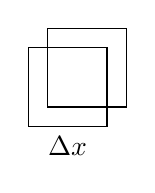
\begin{tikzpicture}
        \draw (0,0) rectangle (1,1);
        \draw (.25,.25) rectangle (1.25,1.25);
        \node [below] at (.5,0) {$\Delta x$};
      \end{tikzpicture}
      \end{paracol}
      \item $(0, +\infty)$. The basis
      \[
        \ab\{\sqrt{\frac2\pi} \cos(kx), \quad \alpha \sim k \in \mathbb R^+\}
      \]
    \end{enumext}
  \end{enumext}
\end{solution}
\begin{problem}[Strum-Liouville theory]
\end{problem}
\begin{solution}[By TA]\leavevmode
  \begin{enumext}
    \item Actually, the problem is something like
    \[
      \braket<u|v> = \int_{x_1}^{x_2} u^*(x) v(x) \omega(x) \d x, \qq{where}
      \alpha(x),\ \beta(x),\ \gamma(x) \in \mathbbm R
    \]
    The operator
    \[
      \mathcal L = \omega^{-1} \odv*[fun]{\omega\alpha \odv*{}x}x + \gamma
    = \alpha \odv*[2]{}x + \omega^{-1} \odv*[fun]{\omega\alpha}x + \gamma
    \]
    Then,
    \[
      \alpha(x)y'' + \beta(x)y' + \gamma(x)y = \lambda y, \quad
      \beta(x) = \omega^{-1} \odv*[fun]{\omega\alpha}x \Rightarrow
      \frac{\beta\omega\alpha}{\alpha} = \odv[fun]{\omega\alpha}x, \Rightarrow
      \omega = \frac C\alpha \upe^{\int\frac\beta\alpha \d x}
    \]
    Or, it can be a extension of the inner product.
    \begin{enumext}[columns = 3]
      \item $\omega(\alpha) = C\upe^{-x^2} \sim \upe^{-x^2}$
      \item $\omega(x) = C \sim 1$.
      \item $\omega(x) = C\upe^{-x} \sim \upe^{-x}$.
    \end{enumext}
    \item Calculate directly
    \[
      \braket<u|\mathcal Lv> = \braket<\mathcal Lu|v>, \quad
      \omega \in \mathbb R
    \]
    Then, we will obtain
    \[
      \mathcal \omega\alpha(u^*v' - u'^*v)\big|_{x_1}^{x_2}, \quad
      \omega(x_2)\alpha(x_2) = \omega(x_1)\alpha(x_1) = 0
    \]
    \begin{enumext}
      \item $(-\infty, +\infty)$
      \[
        H_n(x) = (-1)^n \upe^{x^2} \odv*[n]{\upe^{-x^2}}x, \quad
        \upe^{-t^2+2xt} = \sum_{n=0}^\infty \frac{k\ln(x)}{n!}t^n
      \]
      \item $[-1, 1]$
      \[
        P_n(x) = \frac1{2^nn!} \odv*{(x^2 - 1)^n}x, \quad
        \frac1{\sqrt{t^2 - 2xt + 1}} = \sum_{n=0}^\infty P_n(x)t^n
      \]
      \item 
      \[
        L_n(x) = \frac1{n!} \upe^x \odv*[n,fun]{\upe^{-x} x^n}x, \quad
        \frac1{1 - t} \upe^{-\frac{tx}{1-t}} = \sum_{n=0}^\infty \ln(x) t^n
      \]
    \end{enumext}
    \item Write the eigenfunctions
    \[
      \mathcal Lv_i = \lambda_i v_i, \quad
      \braket<\mathcal Lv_1|v_2> = \braket<v_1|\mathcal Lv_2>
    \]
    then,
    \[
      (\lambda_1 - \lambda_2)\braket<v_1|v_2> = 0, \quad
      \lambda_1 \neq \lambda_2,
      \Rightarrow \braket<v_1|v_2> = 0
    \]
  \end{enumext}
  \begin{remark}
    Actually, an arbitrary function can be exapnded as
    \[
      f(x) = c_01 + c_1 x + c_2 x^2 + \cdots + c_nx^n + \cdots
    \]
    when one write it, he assumed that
    \[
      \{1, x, x^2, x^3, \cdots, x^n, \cdots\}
    \]
    has constructed a basis of $f(x)$. But they are not orthonormal.
    We need to make the orthonormality between every two elements by
    Scimet orthonormality, for example, in range $[0,1]$
    \[
      \int_{A \sim \mathbbm R} \d x \varphi^*(x) \chi(x) = \braket<\varphi|\chi>
    \]
    If the range is $\mathbbm R$, the integral $\int_{\mathbbm R} x^{n+m}$ makes
    no sense. We need to make it square integral on the real axis by
    multiplying, it would be something like a Gaussian function
    $\omega(x) \sim \upe^{-x^2}$. Then, the integral becomes
    \[
      \int_\infty \d x \omega(x) x^{n+m} = 0
    \]
    To ``kill'' the functioin on both sides, or add the weight function
    $\omega = \upe^{-x}$ to kill the function on one side.
  \end{remark}
\end{solution}
\begin{problem}[Linear map]
\end{problem}
\begin{solution}[By TA]\leavevmode
  \begin{enumext}
    \item $L:\ V \to W$. Vector space $f(u)$
    \begin{enumext}
      \item $+$: identity, inverse, commutativity;
      associativity: $(f_1 + f_2) + f_3 = \cdots$
      \item $\times$: $a(bf_1) = (ab)f_1$ 
      \item $+\times$: $a(f_1 + f_2)$, $(a + b)f_1$
    \end{enumext}
    \item $V$ and $W$ are two matrix, the transformation between is a matrix,
    actually, a linear map. The matrix is JUST A TOOL.
    \[
      \bm v = \sum_{i=1}^{\dim(V)} c_i \bm v_i
    \]
    The core formula is
    \[
      f(v_i) = \sum_{j=1}^n w_i F_{ji} \equiv \bm u_i
    \]
    Which can be written into matrix
    \[
      (w_1, w_2, \cdots, w_n)
      \pxmat[showtop = 1, showleft = 1]Fmn =
      (u_1, u_2, \cdots, u_n)
    \]
    Uniqueness: The two vectors are unique, then, the matrix is unique.
    \item For example
    \[
      \begin{pmatrix}
        a & b\\ c& d
      \end{pmatrix} = \sum_{i=1}^4 f_i M_i
      = a\begin{pmatrix}
        1 & 0\\0 & 0
      \end{pmatrix} + b\begin{pmatrix}
        0 & 1\\0 & 0
      \end{pmatrix} + \begin{pmatrix}
        0 & 0\\1 & 0
      \end{pmatrix} + d\begin{pmatrix}
        0 & 0\\0 & 1
      \end{pmatrix}
    \]
    We can write
    \[
      A = \{F^{kl}, 1 \leq k \leq n,\ 1 \leq l \leq m\}, \quad
      F^{kl}(\bm V_i) = \bm W_j \delta_{ik} \delta_{jl}
    \]
    \item By definition
    \begin{align*}
      \ker(f) & = \{v \in V|f(v) = 0\}\\
      \im(f)  & = \{w\in W|w = f(v), v \in V\}\\
      \dim(\ker(f)) & = s, \quad \dim(\im(f)) = m, \quad \dim(V) = g
    \end{align*}
    and prove $s + m = g$.
    We can write
    \[
      S = \{v_1, v_2, \ldots, v_s\}, ~ f(v) = 0, \quad
      M = \{v_{s+1}, \ldots, v_g\},  ~ f(v) = w
    \]
    For arbitrary $v$, $f(v) = 0$, it means a linear combination
    \[
      v = \sum_{i=1}^s c_iv_i, \quad v_i \in S
    \]
    Then, $f(v) = w \in W \Rightarrow v = \sum_{i=g+1}^g c_iv_i$, $v_i \im M$.
    Substitute
    \[
      f(\bm v) = f\ab(\sum_{i=s+1}^g c_i \bm v_i)
    = \sum_{i=s+1}^g c_i f(\bm v_i)
    = \sum_{i=s+1}^g c_i \underbrace{f(\bm v_2)}_{w_i}
    \]
    Then, consider $v_{1 -- 3}$ and $w_{1 -- 3}$. Let
    \[
      w_1 = aw_2 + bw_3, \quad
      f(v_1) = af(v_2) + bf(v_3), \quad = v_1 = av_2 + bv_3
    \]
    Then, we can prove the dim of $W$-space. $s + m = g$.
    \paragraph{Interuption}
    \[
      (w_1, w_2, \cdots, w_n)
      \pxmat[showtop = 1, showleft = 1]Fmn =
      (u_1, u_2, \cdots, u_n)
    \]
    where the top three cols of $F$ is $0$.
  \end{enumext}
  \begin{remark}
    $f:\ V\to W$. The kernel.
    \[
      \ker(f) = \{v\in V|f(v) = 0_w\}
    \]
    conduct the linear space.
    The linear space always is
    \[
      (v, F) = (+, \times)
    \]
    about elements or operations.
    If $v_1$, $v_2 \in \ker(f)$ then $av_1 + bv_2 \in \ker(f)$, $a$, $b \in F$.
    i.e., $\ker$ is a linear space, also,
    the $\im(f) = \{w\in W|\exists u\in V, w = f(u)\} < w$.
    Also, we can separate an arbitrary vector in $V$
    \begin{center}
      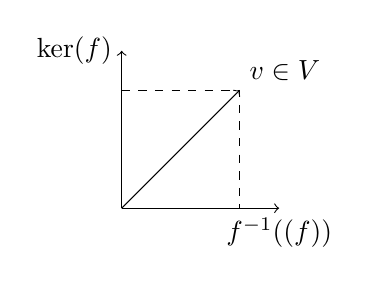
\begin{tikzpicture}
        \draw [->] (0,0) -- (2,0) node [below] {$f^{-1}(\im(f))$};
        \draw [->] (0,0) -- (0,2) node [left] {$\ker(f)$};
        \draw [->] (0,0) -- (1.5,1.5) node [above right] {$v \in V$};
        \draw [dashed] (0,1.5) -- (1.5,1.5) -- (1.5,0);
      \end{tikzpicture}
    \end{center}
  \end{remark}
\end{solution}
\begin{problem}[Coherent states]
\end{problem}
\begin{solution}[By TA]\leavevmode
  \paragraph{Baker-Campbell-Hausdorff}
  \[
    D(\alpha) \equiv \upe^{\alpha\hat a^\dagger - \alpha^*\hat a}
  = \upe^{\alpha\hat a^\dagger} \upe^{-\alpha^*\hat a}
    \upe^{-\frac12[\alpha\hat a^\dagger, \alpha^*\hat a]}
  \]
  \begin{enumext}
    \item By definition
    \[
      \hat a\ket|\alpha> = \alpha\ket|\alpha>
    \]
    Expand it
    \[
      \ket|\alpha> = \sum_{n=0}^\infty c_i \ket|n>
    \]
    Then,
    \[
      \hat a\ket|\alpha> = \sum_{n=0}^\infty c_{n+1} \sqrt{n+1} \ket|n>
    = \alpha \sum_{n=0}^\infty c_n \ket|n>
    \]
    The coefficients
    \[
      c_{n+1}\sqrt{n + 1} = \alpha c_n, \quad
      c_n = \frac{\alpha^n}{\sqrt{n!}} c_0
    \]
    Then, the coherent state can be written as the sum of fork basis
    \[
      \ket|\alpha> = N \sum_{n=0}^\infty \frac{\alpha^n}{\sqrt{n!}} \ket|n>
    \]
    where
    \[
      \ket|n> = \frac1{\sqrt{n!}} (a^\dagger)^n \ket|0>
    \]
    So,
    \[
      \ket|\alpha> = N\sum_{n=0}^\infty
      \frac{(\alpha\hat a^\dagger)^n}{n!}\ket|0>
    \]
    \item Normalization $\braket<\alpha|\alpha>_\alpha = 1$, insert the operator
    \[
      \braket<\hat a^\dagger \hat a|\alpha>
    = (\hat a\ket|\alpha>)^\dagger\hat a\ket|\alpha> = |\alpha|^2
    \]
    Then,
    \[
      \ket|\alpha> = D(\alpha) \ket|0>
    \]
    Finally,
    \[
      \upe^{-\frac12|\alpha|^2\upe^{\alpha\hat a^\dagger}
      \cancelto{\identity}{\upe^{-\alpha^*\hat a}}}\ket|0> \to \identity
    + \hat a
    \]
    \item $\{\ket|\alpha> | \alpha \in \mathbb C\}$ overcomplete.
    $\braket<\alpha|\beta> \neq 0$,
    $\int \frac{\d^2\alpha}{\pi} \ketbra|\alpha><\alpha| = \identity$.
    \[
      \braket<n|\int\frac{\d^2\alpha}{\pi}|\alpha> \braket<\alpha|m>
    = \delta_{nm}
    = \frac1\pi \frac1{\sqrt{n!m!}} \int_0^\infty \d r r^{n+m+1}
      \upe^{-r^2} \int_0^{2\pi} \d\varphi \upe^{\iu\varphi(n-m)}
    = 2\pi\delta_{nm} \xlongequal{n=m} \delta_{nm}
    \]
    \item $\psi_\alpha(x) = \braket<x|\alpha>$.
    \[
      \braket<x|\hat a|\alpha> = \alpha \psi_\alpha(x)
    = \frac1{\sqrt2} \ab(\frac x{l_0} + l_0 \pdif x) \psi_\alpha(x)
    \]
    It is an ODE. The solution is
    \[
      \psi_\alpha(x) = k\exp\ab\{
        \ab(-\frac12\frac x{l_0} - \sqrt2\Re[\alpha])^2
       + \iu\sqrt2\Im[\alpha] \frac x{l_0}\}
    \]
    where $k = (\pi l_0^2)^{-1/4}$.

    The exponitional term
    \[
      \upe^{\frac{(x - x_0)^2}{2\sigma^2} + \iu\frac{p_0}{\hbar}x}
    \]
    The first part means the center of the wavefunction is $x_0$;
    The second term: By Fourier transformation
    \[
      \tilde\psi_\alpha(p)
    = N \int_{-\infty}^\infty \psi_\alpha(x) \upe^{-\iu px/\hbar} \d x
    \propto \upe^{-\frac{(p-p_0)^2}{2\sigma_p^2} + \iu x_0 \frac p\hbar}
    \]
    Means that in the momentum space, centered with $p_0$.
    The position and momentum is closely connected with each other.

    Actually, for coherent state,
    it should be $\upe^{-\frac1{2a}(x - x_c)^2}$ where $a = \Delta x$,
    corresponding to $\Delta p$.
    If define $l_0 = \sqrt{\frac\hbar{m\omega}}$, then $x \sim l_0$,
    $k\sim l_0^{-1}$.
    
    Coherent state vs squeezed state.
    Usually, $\braket<\alpha|\beta> \neq 0$, then define
    $P(\alpha) = |\braket<\alpha|\alpha_0>|^2$.
    The wavepack's centre is (the real part of on $x$ axis,
    or the image part of $k$ axis) $\alpha_0$.
  \end{enumext}
\end{solution}
\begin{problem}[Perturbed harmonic oscillator]
\end{problem}
\begin{solution}[By Li Jian]\leavevmode
  \begin{enumext}
    \item Time-independent:
    $V = \epsilon_0 \hat x
       = \frac{\epsilon_0}{\sqrt2}(\hat a + \hat a^\dagger)$.
    We can consider it as an electric field: the oscillator have a positive
    charge, then the electric potential is gradient.

    In classical situation, just change the equilibirum point.
    In quantum situation, to the exact solution, just merge
    \[
      H = \frac12 m\omega^2 (x - x_0)^2 + C
    \]
    Denote $\hat{\tilde x} = \hat x - x_0$,
    then $[\hat{\tilde x}, \hat k] = \iu$. The annihilation operator
    \[
      \hat{\tilde a} = (\hat x + \iu \hat k)/\sqrt2, \quad
      \hat{\tilde a} \ket|0> = 0, \quad (a^\dagger)^n \ket|0> \sim \ket|n>
    \]
    The matrix element
    \[
      V_{mn} = \braket<m|\hat V|n>
    = V_0(\sqrt n\delta_{m+1,n} + \sqrt m\delta_{m,n+1})
    \]
    After pertubation, the state from ground state
    \[
      \ket|0> \to \ket|g> = \ket|0> + \ket|g^{(1)}> + \ket|g^{(2)}> + \cdots
    \]
    The energy
    \[
      E_g = E_0 + E_g^{(1)} + E_g^{(2)} + \cdots
    \]
    where $E_0 = \frac12\hbar\omega$.
    The result
    \begin{align*}
      E_g^{(1)} & = V_{00} = \braket<0|\hat V|0> = 0,
      \qq{Since the $00$-matrix element is excluded}\\
      E_g^{(2)} & = \sum_{n=1}^\infty -\frac{V_{00} V_{n0}}{E_n - E_0}
    = -\frac{V_0^2}{\hbar\omega}\\
      \ket|g^{(1)}> & = \sum_{n=1}^\infty \ket|n> \ab(-\frac{V_{n0}}{E_n - E_0})
  = -\frac{V_0}{\hbar\omega} \ket|1>\\
      \ket|g^{(2)}> & = \sum_{n=1}^\infty \ket|n>
      \ab[-\frac1{E_n - E_0}\ab(\frac{V_{n0}V_{00}}{E_n - E_0}
    - \sum_{n=1}^\infty \frac{V_{nm}V_{mn}}{E_m - E_0})]
    = \frac1{\sqrt2} \ab(\frac{V_0}{\hbar\omega})^2 \ket|2>
    \end{align*}
    The exact solution: Since the Hamiltonian
    \[
      \hat H = \frac12\hbar\omega\ab[\ab(\frac{\hat x}{l_0})^2 + (l_0\hat k)^2]
    + \sqrt2 V_0 \frac{\hat x}{l_0}
    = \frac12\hbar\omega\ab[\ab
      (\frac{\hat x}{l_0} + \sqrt2\frac{V_0}{\hbar\omega})^2 + (l_0\hat k)^2]
    - \frac{V_0^2}{\hbar\omega}
    \]
    where $l_0 = \sqrt{\frac{\hbar}{m\omega}}$, $V_0 = l_0\epsilon_0/\sqrt2$.
    The ground energy of this Hamiltonian is
    \[
      \tilde E_0 = \underbrace{\frac12 \hbar\omega}_{E_0}
    - \frac{V_0^2}{\hbar\omega}
    \]
    We can consider $\ket|0>$ as a coherent state
    \[
      \hat a\ket|0> = 0\ket|0>
    \]
    The wave function $\upe^{-\frac12(x-0)^2}$,
    $(a^\dagger)^2 \ket|0> = \sqrt2\ket|2>$.
    \[
      \ket|g> = \ket|\alpha = -?\frac{V_0}{\hbar\omega}>
    = \upe^{\alpha\hat a^\dagger} \ket|0>
    = \upe^{-\frac{V_0}{\hbar\omega}a^\dagger} \ket|0>
    = \ket|0> + \ab(-\frac{V_0}{\hbar\omega}\ket|1>)
    + \frac12\ab(-\frac{V_0}{\hbar\omega})^2\sqrt2\ket|2>
    \], i.e., the coherent
    state which center is shifted, and the exact solutions and pertubation
    solutions are corresponding.
    \item To simplify, we need to use the interaction picture
    \[
      V^\text I(t) = \upe^{\frac\iu\hbar\hat H_0t} \hat V^\text S(t)
                     \upe^{-\frac\iu\hbar\hat H_0t}
    = \hbar V(t) (\hat a\upe^{-\iu\omega t} + \hat a^\dagger \upe^{\iu\omega t})
    \]
    where $\hat H_0$ contains $a^\dagger a$ and $\hat V^\text S(t)$
    contains $\hat a + \hat a^\dagger$,
    $v(t) = \frac{\epsilon(t)l_0}{\sqrt2\hbar}$. The coefficient
    \[
      \underset{0\to n}{c_n^{(1)}(t)}
    = -\frac\iu\hbar \int_0^t \d t' \braket<n|\hat V^\text I(t')|0>
    = -\iu\mu_\omega(t) \delta_{n,1}
    \]
    where $\mu_\omega(t) = \int_0^t \d t' v(t') \upe^{\iu\omega t'}$.
    The amplitude of second jump is
    \[
      c_n^{(2)}(t) = (-\frac\iu\hbar)^2 \int_0^t \d t_1 \int_0^{t_1} \d t_2
        \braket<n|\hat V^\text I(t_1)\hat V^\text I(t_2)|0>
    = -\ab[\frac12|\mu_\omega(t)|^2 - \iu C] \delta_{n,0}
    + (-\iu)^2 \frac{\mu_\omega^2(t)}{\sqrt2} \delta_{n,2}
    \]
    At $t = 0$, the evolution of $\ket|0>$ under $\hat U(t)$
    \[
      \ket|0> \xlongrightarrow{\hat U(t)} \ket|?>
    \]
    Since the Heisenberg time-dependent operator
    \[
      \hat a(t) \equiv \hat U(t) \hat a \hat U(t)^{-1} \equiv f_t(\hat a)
    \]
    To solve it, back to the Heisenberg equation
    \[
      \odv*{f_t(\hat a)}t = g_t(\hat a)
    \]
    where $\iu\odv{U(t)}t = HU$, $-\iu\odv{U(t)}t^{-1} = U(t)^{-1}H(t)$.
    It tells
    \[
      \hat a\hat U(t) = \hat U(t) f_t(\hat a)
    \]
    Consider
    \[
      \hat a(\hat U(t)\ket|0>) = \hat U(t) f_t(\hat a) \ket|0>
    = f_t(0) (\hat U(t) \ket|0>)
    \]
    i.e., the exact solution $\ket|\alpha> = \ket|\alpha = f_t(0)>$, and it can
    also be expanded $\sum_n(c_n) \ket|n>$. The eigenvalue of unperturbed state
    is time-dependent $\alpha(t) = -\iu\upe^{-\iu\omega t} \mu_\omega(t)$.
  \end{enumext}
\end{solution}